
\documentclass[border=8pt, multi, tikz]{standalone} 
\usepackage{import}
\subimport{../layers/}{init}
\usetikzlibrary{positioning}
\usetikzlibrary{3d} %for including external image 

\def\ConvColor{rgb:yellow,5;red,2.5;white,5}
\def\ConvReluColor{rgb:yellow,5;red,5;white,5}
\def\PoolColor{rgb:red,1;black,0.3}
\def\UnpoolColor{rgb:blue,2;green,1;black,0.3}
\def\FcColor{rgb:blue,5;red,4;white,5}
\def\FcReluColor{rgb:blue,5;red,5;white,4}
\def\SoftmaxColor{rgb:magenta,5;black,7}   
\def\SumColor{rgb:blue,5;green,15}
\def\Relu{rgb:cyan,5;green,15}
\def\Picture{rgb:blue,5;green,15}
\def\BatchNorm{rgb:pink,5;green,15}
\def\DropoutColor{rgb:magenta,5;black,7}  
\def\LSTMColor{rgb:red,5;black,3}  

\newcommand{\copymidarrow}{\tikz \draw[-Stealth,line width=0.8mm,draw={rgb:blue,4;red,1;green,1;black,3}] (-0.3,0) -- ++(0.3,0);}

\begin{document}
\begin{tikzpicture}
\tikzstyle{connection}=[ultra thick,every node/.style={sloped,allow upside down},draw=\edgecolor,opacity=0.7]
\tikzstyle{copyconnection}=[ultra thick,every node/.style={sloped,allow upside down},draw={rgb:blue,4;red,1;green,1;black,3},opacity=0.7]

\node[canvas is zy plane at x=0] (jedanslika14) at (-3,0,0) {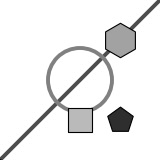
\includegraphics[width=5cm,height=5cm]{../images/slika_1.png}};
\node[below, font=\Large] at (jedanslika14.south) {};

\pic[shift={(2,0,0)}] at (0,0,0) 
    {Box={
        name=jedanconv1,
        caption=,
        xlabel={{32, }},
        zlabel=79,
        fill=\ConvColor,
        height=19,
        width=8,
        depth=19
        }
    };

\pic[shift={(0,0,0)}] at (jedanconv1-east) 
    {Box={
        name=jedannorm1,
        caption=,
        fill=\BatchNorm,
        height=19,
        width=3,
        depth=19
        }
    };

\pic[shift={(0,0,0)}] at (jedannorm1-east) 
    {Box={
        name=jedanrelu1,
        caption=,
        fill=\Relu,
        height=19,
        width=3,
        depth=19
        }
    };

\draw [connection]  (-2, 0, 0)    -- node {\midarrow} (jedanconv1-west);

\pic[shift={(2,0,0)}] at (jedanrelu1-east) 
    {Box={
        name=jedanconv2,
        caption=,
        xlabel={{32, }},
        zlabel=38,
        fill=\ConvColor,
        height=10,
        width=8,
        depth=10
        }
    };

\pic[shift={(0,0,0)}] at (jedanconv2-east) 
    {Box={
        name=jedannorm2,
        caption=,
        fill=\BatchNorm,
        height=10,
        width=3,
        depth=10
        }
    };

\pic[shift={(0,0,0)}] at (jedannorm2-east) 
    {Box={
        name=jedanrelu2,
        caption=,
        fill=\Relu,
        height=10,
        width=3,
        depth=10
        }
    };

\draw [connection]  (jedanrelu1-east)    -- node {\midarrow} (jedanconv2-west);

\pic[shift={(2,0,0)}] at (jedanrelu2-east) 
    {Box={
        name=jedanconv3,
        caption=,
        xlabel={{32, }},
        zlabel=18,
        fill=\ConvColor,
        height=5,
        width=8,
        depth=5
        }
    };

\pic[shift={(0,0,0)}] at (jedanconv3-east) 
    {Box={
        name=jedannorm3,
        caption=,
        fill=\BatchNorm,
        height=5,
        width=3,
        depth=5
        }
    };

\pic[shift={(0,0,0)}] at (jedannorm3-east) 
    {Box={
        name=jedanrelu3,
        caption=,
        fill=\Relu,
        height=5,
        width=3,
        depth=5
        }
    };

\draw [connection]  (jedanrelu2-east)    -- node {\midarrow} (jedanconv3-west);

\pic[shift={(2,0,0)}] at (jedanrelu3-east) 
    {Box={
        name=jedanconv4,
        caption=,
        xlabel={{32, }},
        zlabel=9,
        fill=\ConvColor,
        height=2,
        width=8,
        depth=2
        }
    };

\pic[shift={(0,0,0)}] at (jedanconv4-east) 
    {Box={
        name=jedannorm4,
        caption=,
        fill=\BatchNorm,
        height=2,
        width=3,
        depth=2
        }
    };

\pic[shift={(0,0,0)}] at (jedannorm4-east) 
    {Box={
        name=jedanrelu4,
        caption=,
        fill=\Relu,
        height=2,
        width=3,
        depth=2
        }
    };

\draw [connection]  (jedanrelu3-east)    -- node {\midarrow} (jedanconv4-west);

\pic[shift={(2,0,0)}] at (jedanrelu4-east) 
    {Box={
        name=jedancnn,
        caption=Proces tagovanja,
        zlabel=1,
        fill={rgb: red, 5},
        height=10,
        width=2,
        depth=2
        }
    };

\pic[shift={(0,1.2,0)}] at (jedancnn-west) 
    {Box={
        name=jedantag,
        caption=,
        zlabel=1,
        fill={rgb:red,1;green,2;blue,3},
        height=2,
        width=2,
        depth=2
        }
    };

\draw [connection]  (jedanrelu4-east)    -- node {\midarrow} (jedancnn-west);

\pic[shift={(2,0,0)}] at (jedancnn-east) 
    {Box={
        name=jedanlinear1,
        caption=,
        zlabel=256,
        fill=\FcColor,
        height=10,
        width=2,
        depth=2
        }
    };

\draw [connection]  (jedancnn-east)    -- node {\midarrow} (jedanlinear1-west);

\pic[shift={(2,0,0)}] at (jedanlinear1-east) 
    {Box={
        name=jedanembedded,
        caption=Embeded ,
        zlabel=1,
        fill={rgb:red,0;green,10;blue,0},
        height=2,
        width=10,
        depth=2
        }
    };

\draw [connection]  (jedanlinear1-east)    -- node {\midarrow} (jedanembedded-west);
\node[font=\Large, anchor=west] at (0,6) {\textcolor{black}{Konteksne ploce}};
    \draw [dashed]  (-3,5)    --   (30,5);\node[font=\Large, anchor=west] at (0,4) {\textcolor{black}{Potencijalni odgovori}};
    
\node[canvas is zy plane at x=0] (dvaslika14) at (-3,10,0) {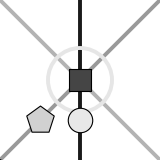
\includegraphics[width=5cm,height=5cm]{../images/slika_2.png}};
\node[below, font=\Large] at (dvaslika14.south) {};

\pic[shift={(2,10,0)}] at (0,0,0) 
    {Box={
        name=dvaconv1,
        caption=,
        xlabel={{32, }},
        zlabel=79,
        fill=\ConvColor,
        height=19,
        width=8,
        depth=19
        }
    };

\pic[shift={(0,0,0)}] at (dvaconv1-east) 
    {Box={
        name=dvanorm1,
        caption=,
        fill=\BatchNorm,
        height=19,
        width=3,
        depth=19
        }
    };

\pic[shift={(0,0,0)}] at (dvanorm1-east) 
    {Box={
        name=dvarelu1,
        caption=,
        fill=\Relu,
        height=19,
        width=3,
        depth=19
        }
    };

\draw [connection]  (-2, 10, 0)    -- node {\midarrow} (dvaconv1-west);

\pic[shift={(2,0,0)}] at (dvarelu1-east) 
    {Box={
        name=dvaconv2,
        caption=,
        xlabel={{32, }},
        zlabel=38,
        fill=\ConvColor,
        height=10,
        width=8,
        depth=10
        }
    };

\pic[shift={(0,0,0)}] at (dvaconv2-east) 
    {Box={
        name=dvanorm2,
        caption=,
        fill=\BatchNorm,
        height=10,
        width=3,
        depth=10
        }
    };

\pic[shift={(0,0,0)}] at (dvanorm2-east) 
    {Box={
        name=dvarelu2,
        caption=,
        fill=\Relu,
        height=10,
        width=3,
        depth=10
        }
    };

\draw [connection]  (dvarelu1-east)    -- node {\midarrow} (dvaconv2-west);

\pic[shift={(2,0,0)}] at (dvarelu2-east) 
    {Box={
        name=dvaconv3,
        caption=,
        xlabel={{32, }},
        zlabel=18,
        fill=\ConvColor,
        height=5,
        width=8,
        depth=5
        }
    };

\pic[shift={(0,0,0)}] at (dvaconv3-east) 
    {Box={
        name=dvanorm3,
        caption=,
        fill=\BatchNorm,
        height=5,
        width=3,
        depth=5
        }
    };

\pic[shift={(0,0,0)}] at (dvanorm3-east) 
    {Box={
        name=dvarelu3,
        caption=,
        fill=\Relu,
        height=5,
        width=3,
        depth=5
        }
    };

\draw [connection]  (dvarelu2-east)    -- node {\midarrow} (dvaconv3-west);

\pic[shift={(2,0,0)}] at (dvarelu3-east) 
    {Box={
        name=dvaconv4,
        caption=,
        xlabel={{32, }},
        zlabel=9,
        fill=\ConvColor,
        height=2,
        width=8,
        depth=2
        }
    };

\pic[shift={(0,0,0)}] at (dvaconv4-east) 
    {Box={
        name=dvanorm4,
        caption=,
        fill=\BatchNorm,
        height=2,
        width=3,
        depth=2
        }
    };

\pic[shift={(0,0,0)}] at (dvanorm4-east) 
    {Box={
        name=dvarelu4,
        caption=,
        fill=\Relu,
        height=2,
        width=3,
        depth=2
        }
    };

\draw [connection]  (dvarelu3-east)    -- node {\midarrow} (dvaconv4-west);

\pic[shift={(2,0,0)}] at (dvarelu4-east) 
    {Box={
        name=dvacnn,
        caption=Proces tagovanja,
        zlabel=1,
        fill={rgb: red, 5},
        height=10,
        width=2,
        depth=2
        }
    };

\pic[shift={(0,1.2,0)}] at (dvacnn-west) 
    {Box={
        name=dvatag,
        caption=,
        zlabel=1,
        fill={rgb:red,1;green,2;blue,3},
        height=2,
        width=2,
        depth=2
        }
    };

\draw [connection]  (dvarelu4-east)    -- node {\midarrow} (dvacnn-west);

\pic[shift={(2,0,0)}] at (dvacnn-east) 
    {Box={
        name=dvalinear1,
        caption=,
        zlabel=256,
        fill=\FcColor,
        height=10,
        width=2,
        depth=2
        }
    };

\draw [connection]  (dvacnn-east)    -- node {\midarrow} (dvalinear1-west);

\pic[shift={(2,0,0)}] at (dvalinear1-east) 
    {Box={
        name=dvaembedded,
        caption=Embeded ,
        zlabel=1,
        fill={rgb:red,10;green,0;blue,0},
        height=2,
        width=10,
        depth=2
        }
    };

\draw [connection]  (dvalinear1-east)    -- node {\midarrow} (dvaembedded-west);
\filldraw[fill=black] (0,0) ++(3,14) circle (0.1);
            \filldraw[fill=black] (0,1) ++(3,14) circle (0.1);
            \filldraw[fill=black] (0,2) ++(3,14) circle (0.1);
            \filldraw[fill=black] (0,0) ++(27,14) circle (0.1);
            \filldraw[fill=black] (0,1) ++(27,14) circle (0.1);
            \filldraw[fill=black] (0,2) ++(27,14) circle (0.1);
            
\node[canvas is zy plane at x=0] (trislika14) at (-3,20,0) {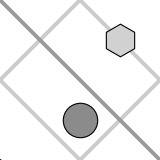
\includegraphics[width=5cm,height=5cm]{../images/slika_3.png}};
\node[below, font=\Large] at (trislika14.south) {};

\pic[shift={(2,20,0)}] at (0,0,0) 
    {Box={
        name=triconv1,
        caption=,
        xlabel={{32, }},
        zlabel=79,
        fill=\ConvColor,
        height=19,
        width=8,
        depth=19
        }
    };

\pic[shift={(0,0,0)}] at (triconv1-east) 
    {Box={
        name=trinorm1,
        caption=,
        fill=\BatchNorm,
        height=19,
        width=3,
        depth=19
        }
    };

\pic[shift={(0,0,0)}] at (trinorm1-east) 
    {Box={
        name=trirelu1,
        caption=,
        fill=\Relu,
        height=19,
        width=3,
        depth=19
        }
    };

\draw [connection]  (-2, 20, 0)    -- node {\midarrow} (triconv1-west);

\pic[shift={(2,0,0)}] at (trirelu1-east) 
    {Box={
        name=triconv2,
        caption=,
        xlabel={{32, }},
        zlabel=38,
        fill=\ConvColor,
        height=10,
        width=8,
        depth=10
        }
    };

\pic[shift={(0,0,0)}] at (triconv2-east) 
    {Box={
        name=trinorm2,
        caption=,
        fill=\BatchNorm,
        height=10,
        width=3,
        depth=10
        }
    };

\pic[shift={(0,0,0)}] at (trinorm2-east) 
    {Box={
        name=trirelu2,
        caption=,
        fill=\Relu,
        height=10,
        width=3,
        depth=10
        }
    };

\draw [connection]  (trirelu1-east)    -- node {\midarrow} (triconv2-west);

\pic[shift={(2,0,0)}] at (trirelu2-east) 
    {Box={
        name=triconv3,
        caption=,
        xlabel={{32, }},
        zlabel=18,
        fill=\ConvColor,
        height=5,
        width=8,
        depth=5
        }
    };

\pic[shift={(0,0,0)}] at (triconv3-east) 
    {Box={
        name=trinorm3,
        caption=,
        fill=\BatchNorm,
        height=5,
        width=3,
        depth=5
        }
    };

\pic[shift={(0,0,0)}] at (trinorm3-east) 
    {Box={
        name=trirelu3,
        caption=,
        fill=\Relu,
        height=5,
        width=3,
        depth=5
        }
    };

\draw [connection]  (trirelu2-east)    -- node {\midarrow} (triconv3-west);

\pic[shift={(2,0,0)}] at (trirelu3-east) 
    {Box={
        name=triconv4,
        caption=,
        xlabel={{32, }},
        zlabel=9,
        fill=\ConvColor,
        height=2,
        width=8,
        depth=2
        }
    };

\pic[shift={(0,0,0)}] at (triconv4-east) 
    {Box={
        name=trinorm4,
        caption=,
        fill=\BatchNorm,
        height=2,
        width=3,
        depth=2
        }
    };

\pic[shift={(0,0,0)}] at (trinorm4-east) 
    {Box={
        name=trirelu4,
        caption=,
        fill=\Relu,
        height=2,
        width=3,
        depth=2
        }
    };

\draw [connection]  (trirelu3-east)    -- node {\midarrow} (triconv4-west);

\pic[shift={(2,0,0)}] at (trirelu4-east) 
    {Box={
        name=tricnn,
        caption=Proces tagovanja,
        zlabel=1,
        fill={rgb: red, 5},
        height=10,
        width=2,
        depth=2
        }
    };

\pic[shift={(0,1.2,0)}] at (tricnn-west) 
    {Box={
        name=tritag,
        caption=,
        zlabel=1,
        fill={rgb:red,1;green,2;blue,3},
        height=2,
        width=2,
        depth=2
        }
    };

\draw [connection]  (trirelu4-east)    -- node {\midarrow} (tricnn-west);

\pic[shift={(2,0,0)}] at (tricnn-east) 
    {Box={
        name=trilinear1,
        caption=,
        zlabel=256,
        fill=\FcColor,
        height=10,
        width=2,
        depth=2
        }
    };

\draw [connection]  (tricnn-east)    -- node {\midarrow} (trilinear1-west);

\pic[shift={(2,0,0)}] at (trilinear1-east) 
    {Box={
        name=triembedded,
        caption=Embeded ,
        zlabel=1,
        fill={rgb:red,0;green,0;blue,10},
        height=2,
        width=10,
        depth=2
        }
    };

\draw [connection]  (trilinear1-east)    -- node {\midarrow} (triembedded-west);

\pic[shift={(32,0,0)}] at (0,0,0) 
    {Box={
        name=embedded1,
        caption=Spojeni parovi latentnih vektora,
        zlabel=1,
        fill={rgb:red,0;green,10;blue,0},
        height=2,
        width=10,
        depth=2
        }
    };

\pic[shift={(0,0,0)}] at (embedded1-east) 
    {Box={
        name=embedded2,
        caption=,
        zlabel=1,
        fill={rgb:red,10;green,0;blue,0},
        height=2,
        width=10,
        depth=2
        }
    };

\pic[shift={(32,3,0)}] at (0,0,0) 
    {Box={
        name=embedded12,
        caption=,
        zlabel=1,
        fill={rgb:red,0;green,10;blue,0},
        height=2,
        width=10,
        depth=2
        }
    };

\pic[shift={(0,0,0)}] at (embedded12-east) 
    {Box={
        name=embedded22,
        caption=,
        zlabel=1,
        fill={rgb:red,0;green,0;blue,10},
        height=2,
        width=10,
        depth=2
        }
    };

\pic[shift={(32,6,0)}] at (0,0,0) 
    {Box={
        name=embedded13,
        caption=,
        zlabel=1,
        fill={rgb:red,10;green,0;blue,0},
        height=2,
        width=10,
        depth=2
        }
    };

\pic[shift={(0,0,0)}] at (embedded13-east) 
    {Box={
        name=embedded23,
        caption=,
        zlabel=1,
        fill={rgb:red,0;green,10;blue,0},
        height=2,
        width=10,
        depth=2
        }
    };
\filldraw[fill=black] (0,0) ++(34,9) circle (0.1);
            \filldraw[fill=black] (0,1) ++(34,9) circle (0.1);
            \filldraw[fill=black] (0,2) ++(34,9) circle (0.1);
            
\pic[shift={(32,14,0)}] at (0,0,0) 
    {Box={
        name=embedded132,
        caption=,
        zlabel=1,
        fill={rgb:red,10;green,0;blue,0},
        height=2,
        width=10,
        depth=2
        }
    };

\pic[shift={(0,0,0)}] at (embedded132-east) 
    {Box={
        name=embedded222,
        caption=,
        zlabel=1,
        fill={rgb:red,0;green,0;blue,10},
        height=2,
        width=10,
        depth=2
        }
    };

\pic[shift={(32,17,0)}] at (0,0,0) 
    {Box={
        name=embedded1321,
        caption=,
        zlabel=1,
        fill={rgb:red,0;green,0;blue,10},
        height=2,
        width=10,
        depth=2
        }
    };

\pic[shift={(0,0,0)}] at (embedded1321-east) 
    {Box={
        name=embedded223,
        caption=,
        zlabel=1,
        fill={rgb:red,10;green,0;blue,0},
        height=2,
        width=10,
        depth=2
        }
    };

\pic[shift={(32,20,0)}] at (0,0,0) 
    {Box={
        name=embedded1322,
        caption=,
        zlabel=1,
        fill={rgb:red,0;green,0;blue,10},
        height=2,
        width=10,
        depth=2
        }
    };

\pic[shift={(0,0,0)}] at (embedded1322-east) 
    {Box={
        name=embedded224,
        caption=,
        zlabel=1,
        fill={rgb:red,0;green,10;blue,0},
        height=2,
        width=10,
        depth=2
        }
    };

\pic[shift={(2,0,0)}] at (embedded2-east) 
    {Box={
        name=linear12,
        caption=,
        zlabel=256,
        fill=\FcColor,
        height=10,
        width=2,
        depth=2
        }
    };

\draw [connection]  (embedded2-east)    -- node {\midarrow} (linear12-west);

\pic[shift={(0,0,0)}] at (linear12-east) 
    {Box={
        name=relu12,
        caption=,
        fill=\Relu,
        height=10,
        width=2,
        depth=2
        }
    };

\pic[shift={(2,0,0)}] at (relu12-east) 
    {Box={
        name=linear13,
        caption=,
        zlabel=256,
        fill=\FcColor,
        height=10,
        width=2,
        depth=2
        }
    };

\draw [connection]  (relu12-east)    -- node {\midarrow} (linear13-west);

\pic[shift={(0,0,0)}] at (linear13-east) 
    {Box={
        name=relu13,
        caption=,
        fill=\Relu,
        height=10,
        width=2,
        depth=2
        }
    };

\pic[shift={(2,0,0)}] at (relu13-east) 
    {Box={
        name=linear14,
        caption=,
        zlabel=256,
        fill=\FcColor,
        height=10,
        width=2,
        depth=2
        }
    };

\draw [connection]  (relu13-east)    -- node {\midarrow} (linear14-west);

\pic[shift={(0,0,0)}] at (linear14-east) 
    {Box={
        name=relu14,
        caption=,
        fill=\Relu,
        height=10,
        width=2,
        depth=2
        }
    };

\pic[shift={(2,0,0)}] at (relu14-east) 
    {Box={
        name=Dropout1,
        caption=\\,
        fill=\DropoutColor,
        height=10,
        width=2,
        depth=2
        }
    };

\draw [connection]  (relu14-east)    -- node {\midarrow} (Dropout1-west);

\pic[shift={(0,0,0)}] at (Dropout1-east) 
    {Box={
        name=relu15,
        caption=,
        fill=\Relu,
        height=10,
        width=2,
        depth=2
        }
    };

\pic[shift={(2,0,0)}] at (embedded22-east) 
    {Box={
        name=linear123,
        caption=,
        zlabel=256,
        fill=\FcColor,
        height=10,
        width=2,
        depth=2
        }
    };

\draw [connection]  (embedded22-east)    -- node {\midarrow} (linear123-west);

\pic[shift={(0,0,0)}] at (linear123-east) 
    {Box={
        name=relu123,
        caption=,
        fill=\Relu,
        height=10,
        width=2,
        depth=2
        }
    };

\pic[shift={(2,0,0)}] at (relu123-east) 
    {Box={
        name=linear124,
        caption=,
        zlabel=256,
        fill=\FcColor,
        height=10,
        width=2,
        depth=2
        }
    };

\draw [connection]  (relu123-east)    -- node {\midarrow} (linear124-west);

\pic[shift={(0,0,0)}] at (linear124-east) 
    {Box={
        name=relu124,
        caption=,
        fill=\Relu,
        height=10,
        width=2,
        depth=2
        }
    };

\pic[shift={(2,0,0)}] at (relu124-east) 
    {Box={
        name=linear125,
        caption=,
        zlabel=256,
        fill=\FcColor,
        height=10,
        width=2,
        depth=2
        }
    };

\draw [connection]  (relu124-east)    -- node {\midarrow} (linear125-west);

\pic[shift={(0,0,0)}] at (linear125-east) 
    {Box={
        name=relu125,
        caption=,
        fill=\Relu,
        height=10,
        width=2,
        depth=2
        }
    };

\pic[shift={(2,0,0)}] at (relu125-east) 
    {Box={
        name=Dropout2,
        caption=\\,
        fill=\DropoutColor,
        height=10,
        width=2,
        depth=2
        }
    };

\draw [connection]  (relu125-east)    -- node {\midarrow} (Dropout2-west);

\pic[shift={(0,0,0)}] at (Dropout2-east) 
    {Box={
        name=relu1261211,
        caption=,
        fill=\Relu,
        height=10,
        width=2,
        depth=2
        }
    };

\pic[shift={(2,0,0)}] at (embedded23-east) 
    {Box={
        name=linear124,
        caption=,
        zlabel=256,
        fill=\FcColor,
        height=10,
        width=2,
        depth=2
        }
    };

\draw [connection]  (embedded23-east)    -- node {\midarrow} (linear124-west);

\pic[shift={(0,0,0)}] at (linear124-east) 
    {Box={
        name=relu124,
        caption=,
        fill=\Relu,
        height=10,
        width=2,
        depth=2
        }
    };

\pic[shift={(2,0,0)}] at (relu124-east) 
    {Box={
        name=linear125,
        caption=,
        zlabel=256,
        fill=\FcColor,
        height=10,
        width=2,
        depth=2
        }
    };

\draw [connection]  (relu124-east)    -- node {\midarrow} (linear125-west);

\pic[shift={(0,0,0)}] at (linear125-east) 
    {Box={
        name=relu125,
        caption=,
        fill=\Relu,
        height=10,
        width=2,
        depth=2
        }
    };

\pic[shift={(2,0,0)}] at (relu125-east) 
    {Box={
        name=linear126,
        caption=,
        zlabel=256,
        fill=\FcColor,
        height=10,
        width=2,
        depth=2
        }
    };

\draw [connection]  (relu125-east)    -- node {\midarrow} (linear126-west);

\pic[shift={(0,0,0)}] at (linear126-east) 
    {Box={
        name=relu126,
        caption=,
        fill=\Relu,
        height=10,
        width=2,
        depth=2
        }
    };

\pic[shift={(2,0,0)}] at (relu126-east) 
    {Box={
        name=Dropout3,
        caption=\\,
        fill=\DropoutColor,
        height=10,
        width=2,
        depth=2
        }
    };

\draw [connection]  (relu126-east)    -- node {\midarrow} (Dropout3-west);

\pic[shift={(0,0,0)}] at (Dropout3-east) 
    {Box={
        name=relu12700,
        caption=,
        fill=\Relu,
        height=10,
        width=2,
        depth=2
        }
    };

\pic[shift={(2,0,0)}] at (embedded222-east) 
    {Box={
        name=linear1254,
        caption=,
        zlabel=256,
        fill=\FcColor,
        height=10,
        width=2,
        depth=2
        }
    };

\draw [connection]  (embedded222-east)    -- node {\midarrow} (linear1254-west);

\pic[shift={(0,0,0)}] at (linear1254-east) 
    {Box={
        name=relu1254,
        caption=,
        fill=\Relu,
        height=10,
        width=2,
        depth=2
        }
    };

\pic[shift={(2,0,0)}] at (relu1254-east) 
    {Box={
        name=linear1264,
        caption=,
        zlabel=256,
        fill=\FcColor,
        height=10,
        width=2,
        depth=2
        }
    };

\draw [connection]  (relu1254-east)    -- node {\midarrow} (linear1264-west);

\pic[shift={(0,0,0)}] at (linear1264-east) 
    {Box={
        name=relu1264,
        caption=,
        fill=\Relu,
        height=10,
        width=2,
        depth=2
        }
    };

\pic[shift={(2,0,0)}] at (relu1264-east) 
    {Box={
        name=linear1274,
        caption=,
        zlabel=256,
        fill=\FcColor,
        height=10,
        width=2,
        depth=2
        }
    };

\draw [connection]  (relu1264-east)    -- node {\midarrow} (linear1274-west);

\pic[shift={(0,0,0)}] at (linear1274-east) 
    {Box={
        name=relu1274,
        caption=,
        fill=\Relu,
        height=10,
        width=2,
        depth=2
        }
    };

\pic[shift={(2,0,0)}] at (relu1274-east) 
    {Box={
        name=Dropout4,
        caption=\\,
        fill=\DropoutColor,
        height=10,
        width=2,
        depth=2
        }
    };

\draw [connection]  (relu1274-east)    -- node {\midarrow} (Dropout4-west);

\pic[shift={(0,0,0)}] at (Dropout4-east) 
    {Box={
        name=relu1275,
        caption=,
        fill=\Relu,
        height=10,
        width=2,
        depth=2
        }
    };

\pic[shift={(2,0,0)}] at (embedded223-east) 
    {Box={
        name=linear12612,
        caption=,
        zlabel=256,
        fill=\FcColor,
        height=10,
        width=2,
        depth=2
        }
    };

\draw [connection]  (embedded223-east)    -- node {\midarrow} (linear12612-west);

\pic[shift={(0,0,0)}] at (linear12612-east) 
    {Box={
        name=relu12612,
        caption=,
        fill=\Relu,
        height=10,
        width=2,
        depth=2
        }
    };

\pic[shift={(2,0,0)}] at (relu12612-east) 
    {Box={
        name=linear12712,
        caption=,
        zlabel=256,
        fill=\FcColor,
        height=10,
        width=2,
        depth=2
        }
    };

\draw [connection]  (relu12612-east)    -- node {\midarrow} (linear12712-west);

\pic[shift={(0,0,0)}] at (linear12712-east) 
    {Box={
        name=relu12712,
        caption=,
        fill=\Relu,
        height=10,
        width=2,
        depth=2
        }
    };

\pic[shift={(2,0,0)}] at (relu12712-east) 
    {Box={
        name=linear12712,
        caption=,
        zlabel=256,
        fill=\FcColor,
        height=10,
        width=2,
        depth=2
        }
    };

\draw [connection]  (relu12712-east)    -- node {\midarrow} (linear12712-west);

\pic[shift={(0,0,0)}] at (linear12712-east) 
    {Box={
        name=relu12712,
        caption=,
        fill=\Relu,
        height=10,
        width=2,
        depth=2
        }
    };

\pic[shift={(2,0,0)}] at (relu12712-east) 
    {Box={
        name=Dropout5,
        caption=\\,
        fill=\DropoutColor,
        height=10,
        width=2,
        depth=2
        }
    };

\draw [connection]  (relu12712-east)    -- node {\midarrow} (Dropout5-west);

\pic[shift={(0,0,0)}] at (Dropout5-east) 
    {Box={
        name=relu12713,
        caption=,
        fill=\Relu,
        height=10,
        width=2,
        depth=2
        }
    };

\pic[shift={(2,0,0)}] at (embedded224-east) 
    {Box={
        name=linear12742,
        caption=,
        zlabel=256,
        fill=\FcColor,
        height=10,
        width=2,
        depth=2
        }
    };

\draw [connection]  (embedded224-east)    -- node {\midarrow} (linear12742-west);

\pic[shift={(0,0,0)}] at (linear12742-east) 
    {Box={
        name=relu12742,
        caption=,
        fill=\Relu,
        height=10,
        width=2,
        depth=2
        }
    };

\pic[shift={(2,0,0)}] at (relu12742-east) 
    {Box={
        name=linear12742,
        caption=,
        zlabel=256,
        fill=\FcColor,
        height=10,
        width=2,
        depth=2
        }
    };

\draw [connection]  (relu12742-east)    -- node {\midarrow} (linear12742-west);

\pic[shift={(0,0,0)}] at (linear12742-east) 
    {Box={
        name=relu12742,
        caption=,
        fill=\Relu,
        height=10,
        width=2,
        depth=2
        }
    };

\pic[shift={(2,0,0)}] at (relu12742-east) 
    {Box={
        name=linear12742,
        caption=,
        zlabel=256,
        fill=\FcColor,
        height=10,
        width=2,
        depth=2
        }
    };

\draw [connection]  (relu12742-east)    -- node {\midarrow} (linear12742-west);

\pic[shift={(0,0,0)}] at (linear12742-east) 
    {Box={
        name=relu12742,
        caption=,
        fill=\Relu,
        height=10,
        width=2,
        depth=2
        }
    };

\pic[shift={(2,0,0)}] at (relu12742-east) 
    {Box={
        name=Dropout6,
        caption=\\,
        fill=\DropoutColor,
        height=10,
        width=2,
        depth=2
        }
    };

\draw [connection]  (relu12742-east)    -- node {\midarrow} (Dropout6-west);

\pic[shift={(0,0,0)}] at (Dropout6-east) 
    {Box={
        name=relu12743,
        caption=,
        fill=\Relu,
        height=10,
        width=2,
        depth=2
        }
    };

\pic[shift={(55,9,0)}] at (0,0,0) 
    {Ball={
        name=sum1,
        fill=\SumColor,
        opacity=0.6,
        radius=3.5,
        logo=$+$
        }
    };

\draw [connection]  (relu15-east)    -- node {\midarrow} (sum1-west);

\draw [connection]  (relu1261211-east)    -- node {\midarrow} (sum1-west);

\draw [connection]  (relu12700-east)    -- node {\midarrow} (sum1-west);

\draw [connection]  (relu1275-east)    -- node {\midarrow} (sum1-west);

\draw [connection]  (relu12713-east)    -- node {\midarrow} (sum1-west);

\draw [connection]  (relu12743-east)    -- node {\midarrow} (sum1-west);

\pic[shift={(2,0,0)}] at (sum1-east) 
    {Box={
        name=embedded3233,
        caption=Embeded ,
        zlabel=256,
        fill={rgb:red,7;green,2;blue,3},
        height=2,
        width=10,
        depth=2
        }
    };

\draw [connection]  (sum1-east)    -- node {\midarrow} (embedded3233-west);

\end{tikzpicture}
\end{document}
